\documentclass[11pt]{beamer}
\usetheme{Madrid}
\usepackage[utf8]{inputenc}
\usepackage{amsmath, amssymb, amsfonts, amsthm}
\usepackage{xcolor}

\usepackage{tikz-cd}
%\usepackage{enumitem}

\author[\texttt{sebastiano.tronto@uni.lu}]{Sebastiano Tronto}
\title{More Latex}
\logo{
\includegraphics[scale=0.1]{img/unilu.jpg}} 
%\institute{University of Luxembourg} 

\newcommand{\bs}{\textbackslash}

\date{2021-03-12} 

\begin{document}

\begin{frame}
  \titlepage
\end{frame}

\begin{frame}{Theorems (review)}
  \begin{center}
    \large
    \texttt{\bs newtheorem\{env-name\}{\color{red}[number-with]}\{Text\}{\color{red}[number-parent]}}
  \end{center}

  \vspace{0.4cm}
  \begin{itemize}
    \item \texttt{env-name}: Environment name (use
          \texttt{\bs begin\{env-name\}...})
    \item \texttt{Text}: Theorem name to be displayed
    \item \texttt{[number-with]} for ``shared counter''
    \item \texttt{[number-parent]} adds x.1
    \item {\color{red} At most one of \texttt{[number-with]}
           and \texttt{[number-parent]}}
  \end{itemize}
  
\end{frame}

\begin{frame}{Theorems (review)}
  \begin{columns}
    \column{0.5\textwidth}
      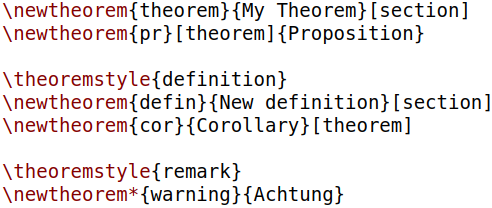
\includegraphics[scale=0.3]{img/thm_pre.png}

      \vspace{0.2cm}
      \vdots
      \vspace{0.3cm}

      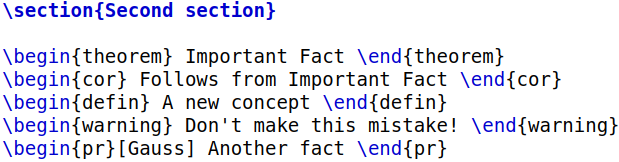
\includegraphics[scale=0.3]{img/thm_tex.png}

    \column{0.5\textwidth}
      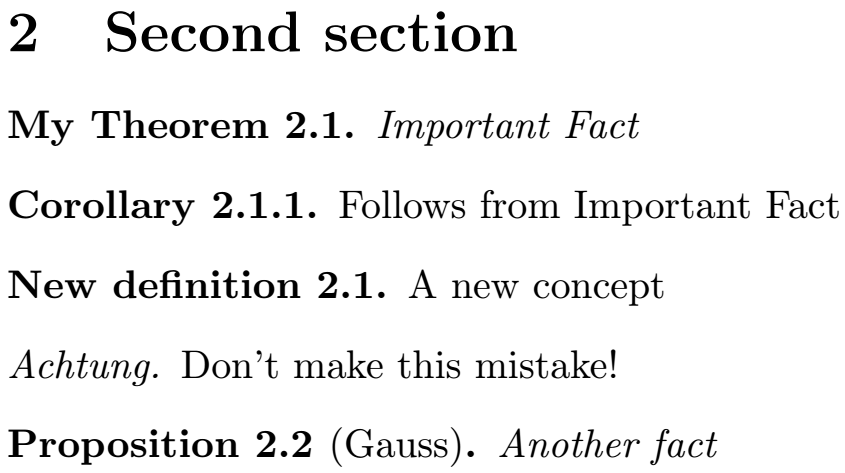
\includegraphics[scale=0.2]{img/thm_pdf.png}

      \vspace{1cm}
  \end{columns}
\end{frame}


\begin{frame}{Counters}
  Reference: \url{https://en.wikibooks.org/wiki/LaTeX/Counters}

  \vspace{0.5cm}
  \begin{itemize}
    \item Sections, theorems etc have an associated \emph{counter}

    \vspace{0.2cm}
    \item Common usage:

          \vspace{0.1cm}
          \texttt{\bs setcounter\{counter-name\}\{n\} \quad \%Set counter to n}

          \vspace{0.1cm}
          \texttt{\bs addtocounter\{counter-name\}\{n\}\quad\%Add n to counter}
  \end{itemize}
\end{frame}


\begin{frame}{Counters}
  
  \begin{itemize}
    \item Define a counter with \texttt{\bs newcounter\{name\}[number-parent]}

    \vspace{0.2cm}
    \item Change sub-numbering of defined counters:

          \vspace{0.15cm}
          \begin{center}
            \begin{tabular}{l}
              \texttt{\bs numberwithin\{equation\}\{section\}}
              %\texttt{\bs numberwithout\{subsection\}\{section\}}
            \end{tabular}
          \end{center}

    \vspace{0.2cm}
    \item Print formatted counter with \texttt{\bs{\color{red}the}name}
          or just number with \texttt{\bs arabic\{name\}}
          (or \texttt{\bs alph}, \texttt{\bs Alph}, \texttt{\bs roman}, 
          \texttt{\bs Roman}, \texttt{\bs fnsymbol})
  \end{itemize}
\end{frame}


\begin{frame}{Counters}
  
  \begin{columns}
    
    \column{0.5\textwidth}
    \begin{center}
      {\large\textbf{Default counters}}
  
      \vspace{0.3cm}
      \begin{tabular}{l}
        %part \\
        chapter \\
        section \\
        subsection \\
        subsubsection \\
        paragraph \\
        %subparagraph \\
        page \\
        figure \\
        %table \\
        footnote \\
        %mpfootnote \\
        equation \\
        enumi \\
        enumii \\
        ...
        %enumiii \\
        %enumiv \\
      \end{tabular}
    \end{center}

    \column{0.5\textwidth}
    {\large\textbf{Counter styles}}

    \vspace{0.3cm}
    \begin{tabular}{ll}
      \texttt{arabic} & 1, 2, 3, 4... \\
      \texttt{alph}   & a, b, c, d... \\
      \texttt{Alph}   & A, B, C, D... \\
      \texttt{roman}  & i, ii, iii, iv... \\
      \texttt{Roman}  & I, II, III, IV... \\
      \texttt{fnsymbol} & $\ast$, $\dagger$, $\ddagger$, $\S$ ...
    \end{tabular}
  \end{columns}
\end{frame}

\begin{frame}{Counters: change \texttt{\bs thecounter}}
  \begin{itemize}
    \item Change how counter is displayed by default, for example:

          \vspace{0.2cm}
          \begin{center}
            \texttt{\bs renewcommand\{\bs thesection\}\{\bs alph\{section\}\}}
          \end{center}

    \vspace{0.3cm}
    \item For enumerate:

          \vspace{0.2cm}
          \begin{center}
            \begin{tabular}{l}
              \texttt{\bs usepackage\{enumitem\}} \\
              \texttt{\bs begin\{enumerate\}[label=\bs alph*]}
            \end{tabular}
          \end{center}
  \end{itemize}
\end{frame}

\begin{frame}{\texttt{label} and \texttt{ref}}
  \begin{itemize}
    \item Put \texttt{\bs label\{mark\}} immediately after the thing you want
          to refer to (after \texttt{\bs refstepcounter\{countername\}} for
          counters you define)

    \vspace{0.3cm}
    \item Use \texttt{\bs ref\{mark\}} or \texttt{\bs eqref\{mark\}} to refer
          %(or \texttt{\bs eqref\{mark\}} = \texttt{(\bs ref\{mark\})})

          (Pro tip: write \texttt{Proposition$\sim$\bs ref\{mark\}})
    \vspace{0.3cm}
    \item Compile twice!
  \end{itemize}
\end{frame}


\begin{frame}{The \texttt{hyperref} package}
  \texttt{\bs usepackage\{hyperref\}}

  \vspace{1cm}
  \begin{itemize}
    \item Now all \texttt{\bs ref\{mark\}} become clickable!

    \vspace{0.3cm}
    \item \texttt{\bs hyperref[mark]\{text\}} for internal links

    \vspace{0.3cm}
    \item \texttt{\bs url\{www.google.com\}} or
          \texttt{\bs href\{www.google.com\}\{Google\}} for web links
  \end{itemize}
\end{frame}

\begin{frame}{New commands}
  \begin{itemize}
    \item We have seen \texttt{\bs newcommand\{\bs command\}\{output\}}

    \vspace{0.3cm}
    \item Arguments: use \texttt{\bs newcommand\{\bs command\}[n]\{output\}}
          and use the arguments in \texttt{output} with
          \texttt{\#1, \#2, ... \#n} \hspace{0.4cm}(\texttt n$\leq 9$)

    \vspace{0.3cm}
    \item If \texttt{\bs command} is already defined:
          \texttt{\bs renewcommand} (overwrite) or
          \texttt{\bs providecommand} (use old definition, if it exists)
  \end{itemize}
\end{frame}

\begin{frame}{New commands - examples}
  
  \begin{tabular}{l|c}
    \texttt{\bs newcommand\{hi\}\{Hello, World!\}} \\
    \texttt{\bs hi} & Hello, world! \\
    \\
    \texttt{\bs newcommand\{hello\}[1]\{Hello, \#1!\}} \\
    \texttt{\bs hello\{my friend\}} & Hello, my friend! \\
    \\
    \texttt{\bs renewcommand\{binom\}[2]\{bin(\#1,\#2)\}} \\
    \texttt{\bs( \bs binom\{10\}2 \bs)} & \(bin(10,2)\)
  \end{tabular}
\end{frame}


\begin{frame}{New commands - optional argument}
  \texttt{\bs newcommand\{\bs com\}[n][default1]\{output\}}

  \texttt{\bs com[first]\{other,args\}} or \texttt{\bs com\{without,first\}}

  \vspace{1cm}
  \begin{itemize}
    \item At most one optional argument, must be \texttt{\# 1}

    \vspace{0.3cm}
    \item More complex things: use TeX primitives such as
          \texttt{\bs ifthenelse} or see
          \url{https://www.ctan.org/tex-archive/support/newcommand/}
  \end{itemize}
\end{frame}

\begin{frame}{Exercises}
  \begin{enumerate}%[label=(\arabic*)]
    \item Write a command \texttt{\bs mat} which takes $4$ arguments and
          outputs a $2\times 2$ matrix with those arguments as entries
          (use \texttt{pmatrix}).

    \vspace{0.5cm}
    \item Write a command to define a function case-by-case ($2$ cases,
          $4$ arguments). Use the \texttt{cases} environment:

          \vspace{0.2cm}
          \begin{columns}
            \column{0.45\textwidth}
            \begin{center}\begin{tabular}{l}
              \texttt{\bs begin\{cases\}} \\
              \texttt{\quad 1 \& 2 \bs\bs \quad3 \& 4} \\
              \texttt{\bs end\{cases\}}
            \end{tabular}\end{center}

            \column{0.09\textwidth}
              \begin{center} $\implies$ \end{center}

            \column{0.45\textwidth}
            \begin{align*}
              \begin{cases} 1 & 2 \\ 3 & 4 \end{cases}
            \end{align*}
          \end{columns}
  \end{enumerate}
\end{frame}


\begin{frame}{Pictures}
  \texttt{\bs usepackage\{graphicx\}} 

  \texttt{\bs includegraphics[options]\{picture.jpg\}} 

  \vspace{1cm}
  Options (comma-separated) include:

  \vspace{0.2cm}
  \begin{itemize}
    \item \texttt{scale=x} (scale by a factor of x)
    \item \texttt{width=x} and \texttt{height=y} (if both specified picture
          is distorted)
    \item \texttt{angle=$\alpha$} (rotate)
  \end{itemize}
\end{frame}


\begin{frame}{Figures}
  \texttt{\bs begin\{figure\}[place]}
  
  \vspace{1cm}
  \begin{itemize}
    \item Figure outside normal text flow.
    \item \texttt{place}: \texttt{h} (here), \texttt{t} (top) or \texttt{b}
          (bottom).
    \item Can add \emph{caption}
  \end{itemize}

  \vspace{0.3cm}
  \begin{center} \begin{tabular}{l}
    \texttt{\bs begin\{figure\}[h]} \\
    \texttt{\qquad\bs centering \qquad \% recommended} \\
    \texttt{\qquad \bs includegraphics\{picture.jpg\}} \\
    \texttt{\qquad \bs caption\{Description of the picture\}} \\
    \texttt{\bs end\{figure\}}
  \end{tabular} \end{center}
\end{frame}


\begin{frame}{Wrapping text around figures}

 \texttt{\bs usepackage\{{\color{red}wrapfig}\}}

  \texttt{\bs begin\{wrapfigure\}{\color{red}\{alignment\}\{width\}}}
  
  \vspace{1cm}
  \begin{itemize}
    \item \texttt{alignment}: \texttt{l} (left) or \texttt{r} (right)
    \item Must specify \texttt{width}
    \item Works the same as \texttt{figure}
  \end{itemize}

  \vspace{0.3cm}
  \begin{center} \begin{tabular}{l}
    \texttt{\bs begin\{wrapfigure\}{\color{red}\{l\}\{0.5\bs textwidth\}}} \\
    \texttt{\qquad\bs centering} \\
    \texttt{\qquad \bs includegraphics\{picture.jpg\}} \\
    \texttt{\qquad \bs caption\{Description of the picture\}} \\
    \texttt{\bs end\{wrapfigure\}}
  \end{tabular} \end{center}
\end{frame}


\begin{frame}{Lengths}
  Reference: \url{https://en.wikibooks.org/wiki/LaTeX/Lengths}

  \vspace{0.5cm}
  \begin{itemize}
    \item Similar to counters:

          \vspace{0.3cm}
          \begin{center}\begin{tabular}{l}
            \texttt{\bs newlength\{\bs lengthname\}}\\
            \texttt{\bs setlength\{\bs lengthname\}\{value\}}
          \end{tabular}\end{center}
          
    \vspace{0.3cm}
    \item \texttt{value}: number followed by unit
          (\texttt{12pt}, \texttt{1.2cm}, \texttt{65mm}, \dots)
  \end{itemize}
\end{frame}

\begin{frame}{Lengths}
  Default lengths:

  \vspace{0.5cm}
  \begin{itemize}
    \item \texttt{\bs textwidth}: width of text in a page
    \item \texttt{\bs textheight}: height of text in a page
    \item \texttt{\bs baselineskip}: space between lines in same paragraph
    \item \texttt{\bs parskip}: space between paragraphs
    \item \texttt{\bs parindent}: indentation of first line of a paragraph
    \item \dots
  \end{itemize}
\end{frame}

\begin{frame}{Manual spacing}
  \begin{itemize}
    \item \texttt{\bs vspace\{length\}} and \texttt{\bs hspace\{length\}}

    \vspace{0.2cm}
    \item Fill space: \texttt{\bs vfill} and \texttt{\bs hfill}

    \vspace{0.2cm}
    \item Fill line with ``decoration'':
          \texttt{\bs hrulefill} and \texttt{\bs dotfill}

    \vspace{0.2cm}
    \item Example:
    
          \vspace{0.2cm}
          \begin{center}
          \texttt{First name: \bs hrulefill \bs quad Last name: \bs hrulefill}
          \end{center}
  \end{itemize}
\end{frame}



\begin{frame}{Bibliography}
  Simple bibliography with \texttt{thebibliography} environment:

  \vspace{0.5cm}
  \begin{center}\begin{tabular}{l}
    \texttt{\bs begin\{thebibliography\}\{99\}} \\
    \texttt{\qquad\bs bibitem\{knuth68\}} \\
    \texttt{\qquad\qquad Donald Knuth, The Art of Computer Programming,} \\
    \texttt{\qquad\qquad Volume I, 1968, Addison-Wesley}\\
    \texttt{\bs end\{thebibliography\}}
  \end{tabular}\end{center}

  %\vspace{0.5cm}
  %And cite with \texttt{\bs cite\{knuth68\}}
\end{frame}


\begin{frame}{Bibligraphy}
  \begin{itemize}
    \item Simple citation: \texttt{\bs cite\{knuth68\}}

    \vspace{0.3cm}
    \item Cite multiple sources: \texttt{\bs cite\{source1, source2\}}

    \vspace{0.3cm}
    \item Cite specific part with \texttt{\bs cite[p.$\sim$42]\{source\}}
  \end{itemize}
\end{frame}


\begin{frame}{Bibliography: BibTeX}
  \begin{itemize}
    \item Separate file \texttt{mybib.bib}, different syntax:

          \begin{center}\begin{tabular}{l}
            \texttt{@book\{knuth68,} \\
            \texttt{\qquad author    = "Donald Knuth",}\\
            \texttt{\qquad title     = "The Art of Computer Programming",}\\
            \texttt{\qquad publisher = "Addison-Wesley",}\\
            \texttt{\qquad volume    = "I",}\\
            \texttt{\qquad year      = "1968",} \\
            \texttt{\}}
          \end{tabular}\end{center}

    \vspace{0.3cm}
    \item Include bibliography in your \texttt{.tex} file:

          \begin{center}\begin{tabular}{l}
            \texttt{\bs bibliographystyle\{plain\}}\\
            \texttt{\bs bibliography\{mybib\}}
          \end{tabular}\end{center}
  \end{itemize}
\end{frame}


\begin{frame}{Bibliography: BibTeX}
  \begin{itemize}
    \item Compile, generate bibliography, compile, compile

    \vspace{0.3cm}
    \item Books in \texttt{.bib} file but not cited do not appear

    \vspace{0.3cm}
    \item Citing articles and other: see \url{https://en.wikibooks.org/wiki/%
          LaTeX/Bibliography\_Management\#Standard\_templates}

    \vspace{0.3cm}
    \item Find BibTeX citations on \url{https://scholar.google.com}
  \end{itemize}
\end{frame}

\end{document}

